\documentclass[11pt]{article}
\usepackage{matt}
\begin{document}

\section*{Update for the Week of \today (Power-Law Quasar Continuum Fits)}

The continuum fits using a power law extrapolated from the red side of \lya\ appear to be very dissimilar to those from quasar templates. Maybe you are using the wrong power in the power-law fit? Worth checking.

\begin{figure}[h]
  \centering
  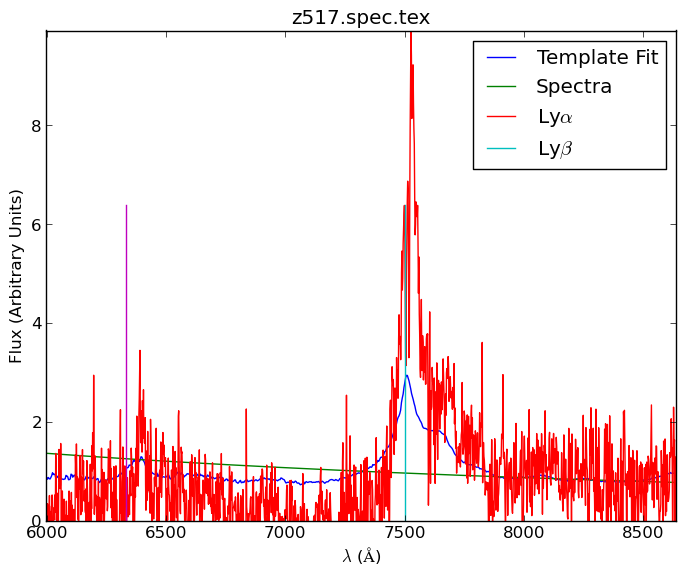
\includegraphics[width=8cm]{z517_spec.png}
  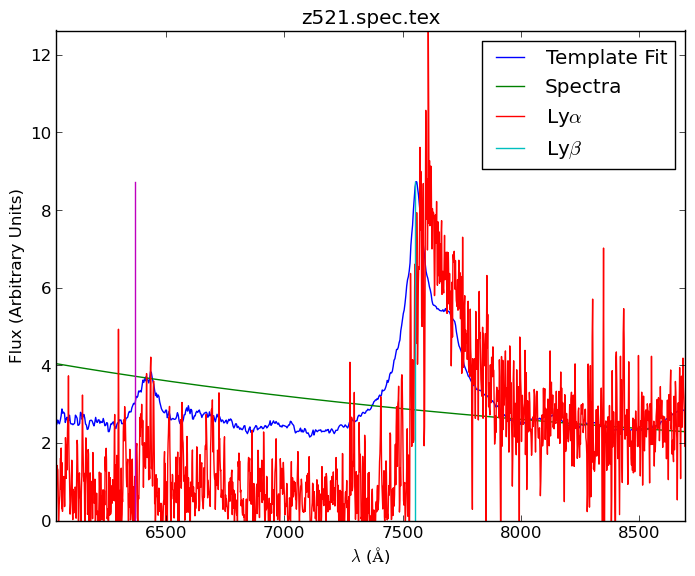
\includegraphics[width=8cm]{z521_spec.png}
  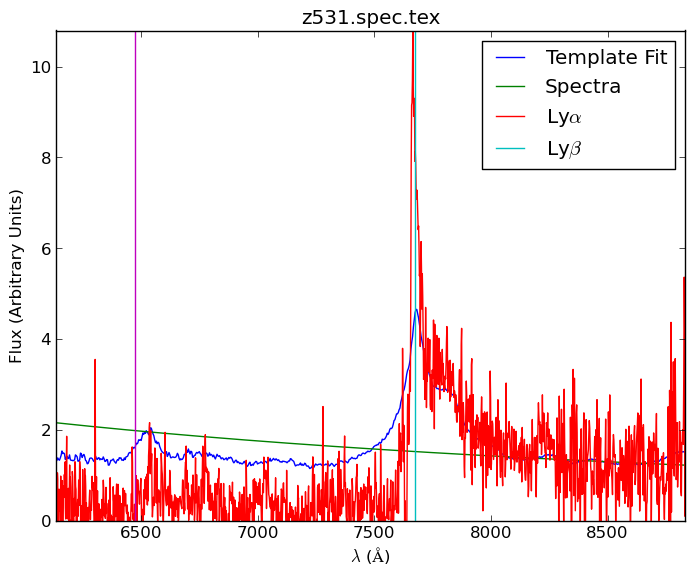
\includegraphics[width=8cm]{z531_spec.png}
  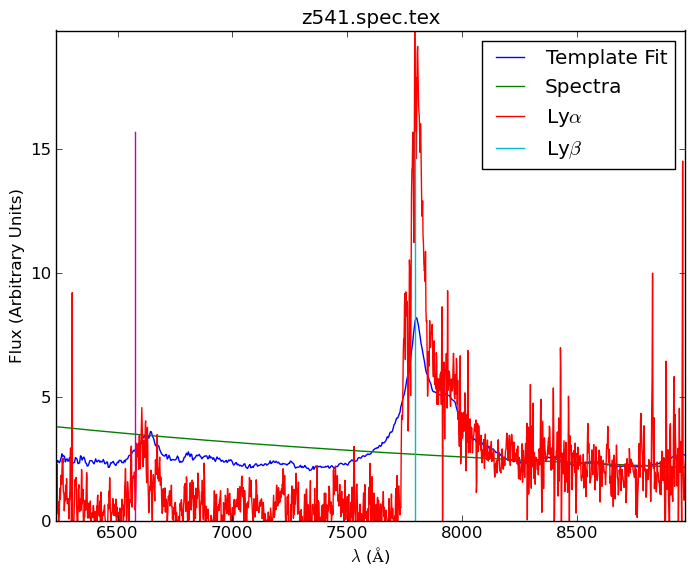
\includegraphics[width=8cm]{z541_spec.png}
  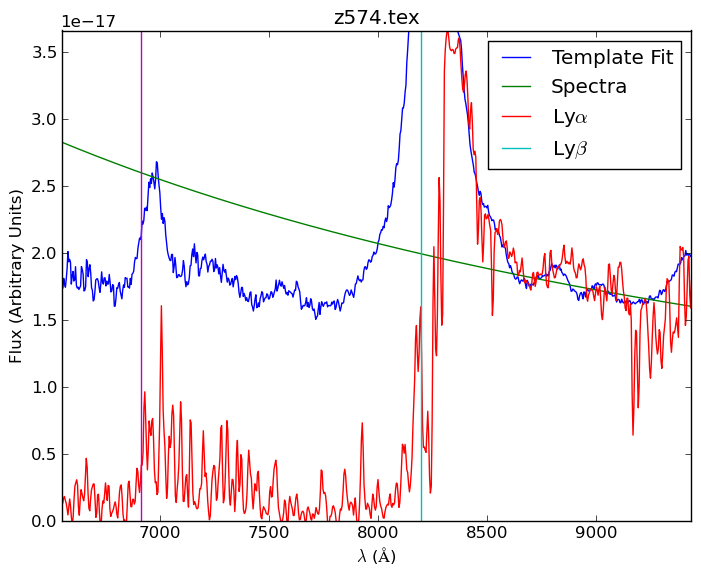
\includegraphics[width=8cm]{z574.png}
  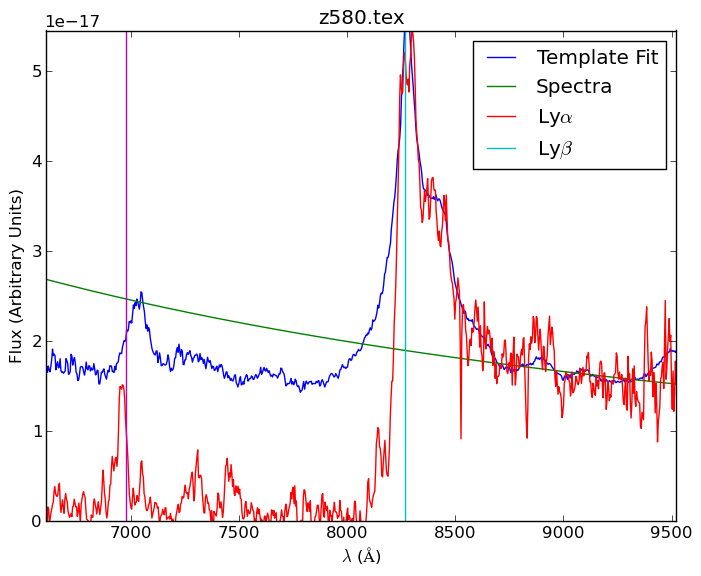
\includegraphics[width=8cm]{z580.png}
  \caption{todo}
  \label{fig:todo}
\end{figure}

\begin{figure}[h]
  \centering
  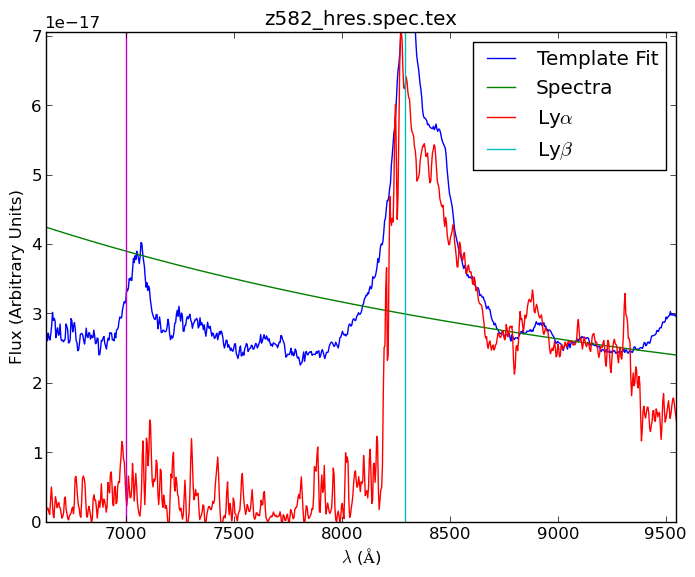
\includegraphics[width=8cm]{z582_hres_spec.png}
  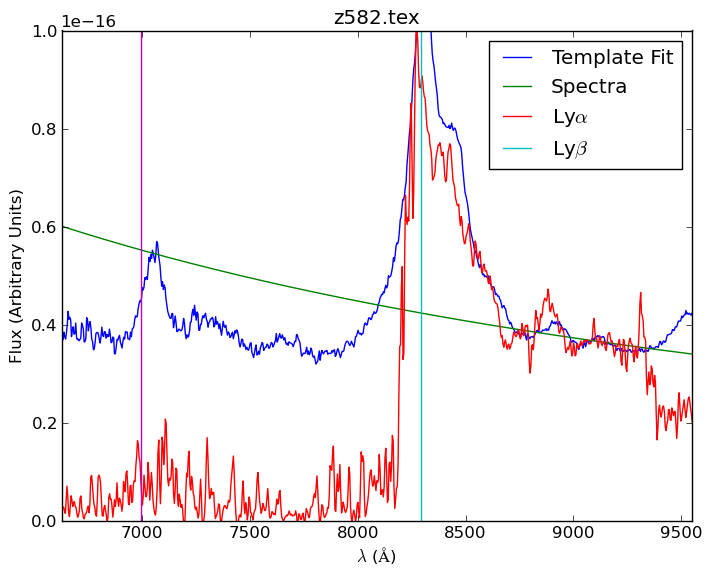
\includegraphics[width=8cm]{z582.png}
  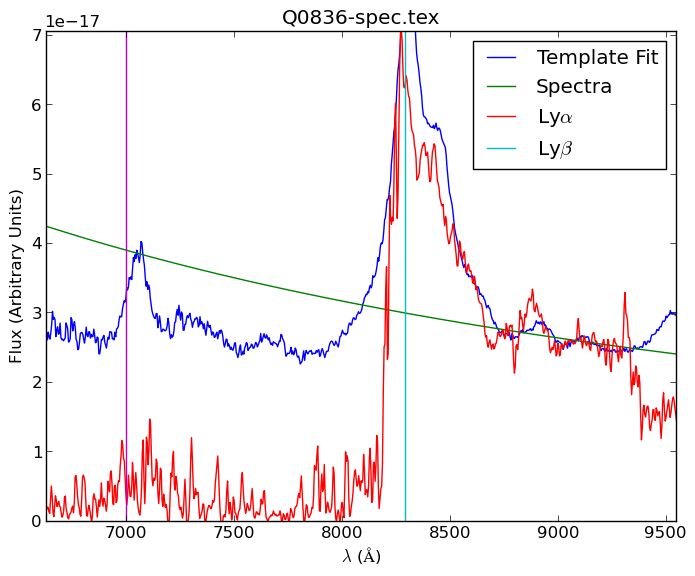
\includegraphics[width=8cm]{Q0836-spec.png}
  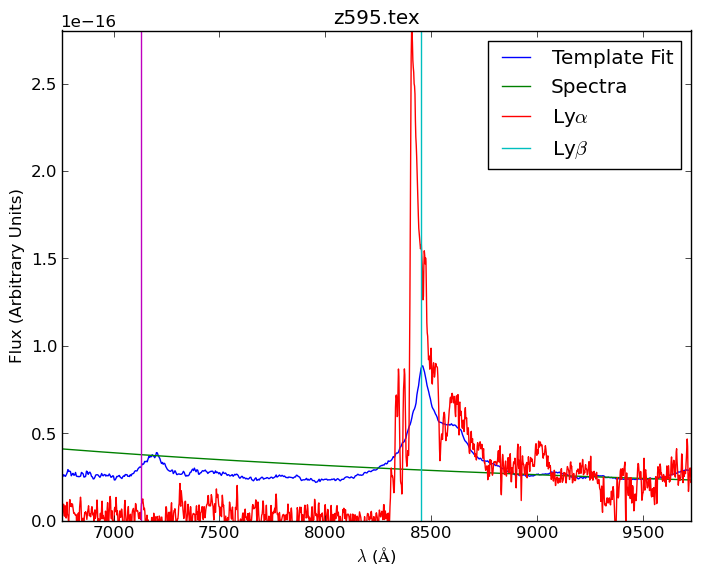
\includegraphics[width=8cm]{z595.png}
  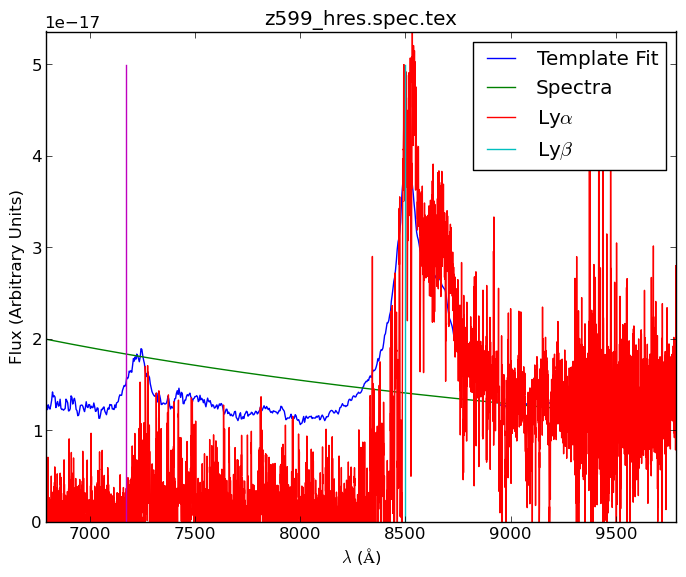
\includegraphics[width=8cm]{z599_hres_spec.png}
  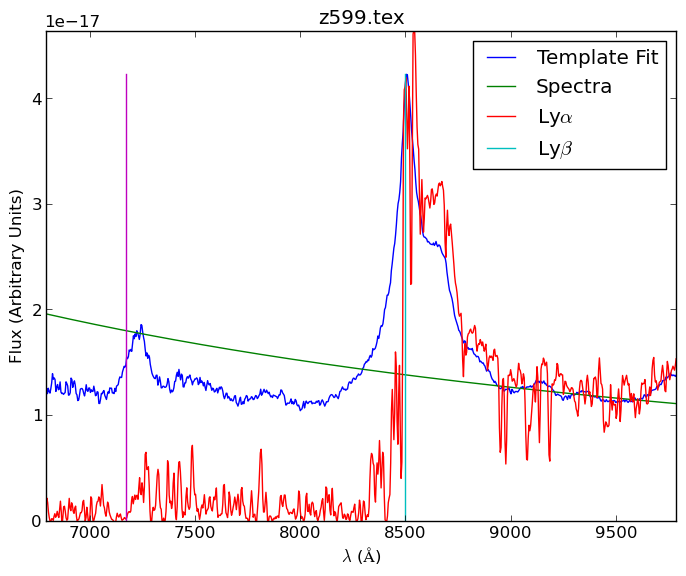
\includegraphics[width=8cm]{z599.png}
  \caption{todo}
  \label{fig:todo}
\end{figure}

\begin{figure}[h]
  \centering
  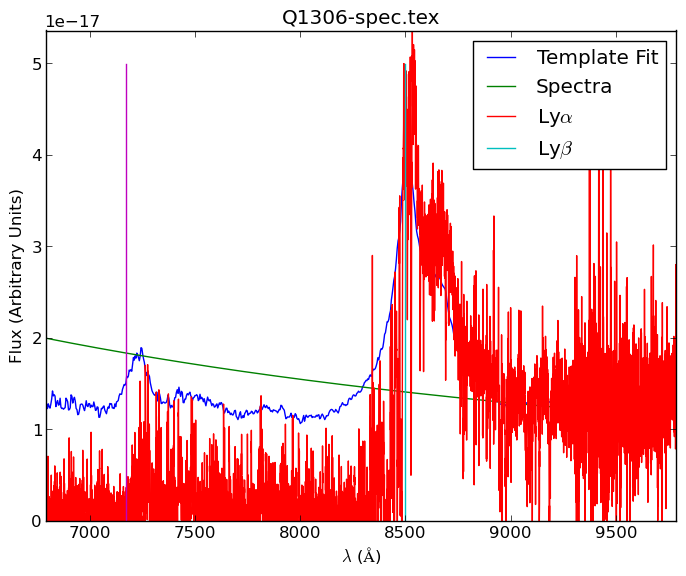
\includegraphics[width=8cm]{Q1306-spec.png}
  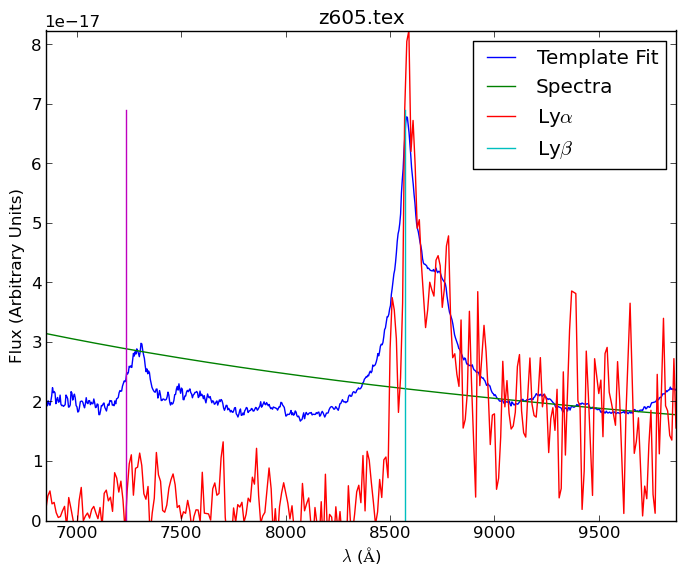
\includegraphics[width=8cm]{z605.png}
  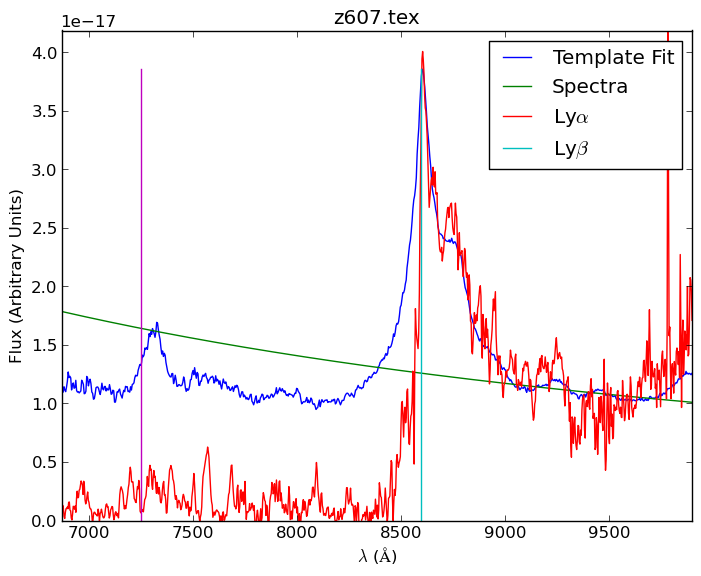
\includegraphics[width=8cm]{z607.png}
  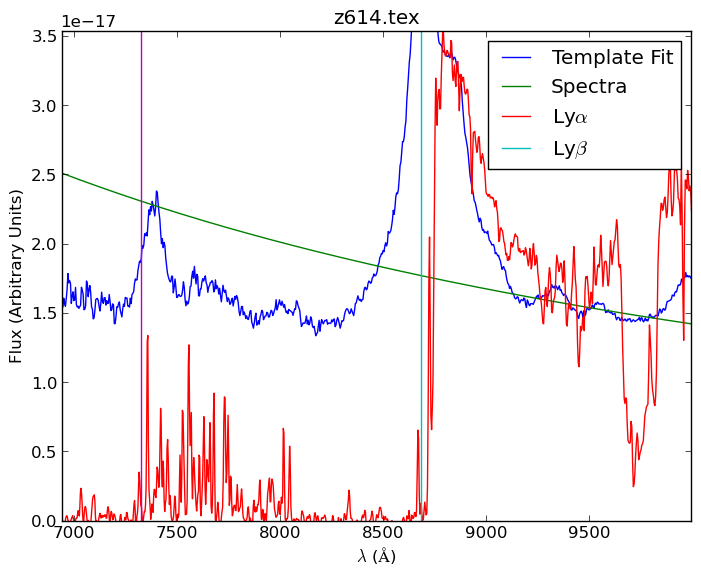
\includegraphics[width=8cm]{z614.png}
  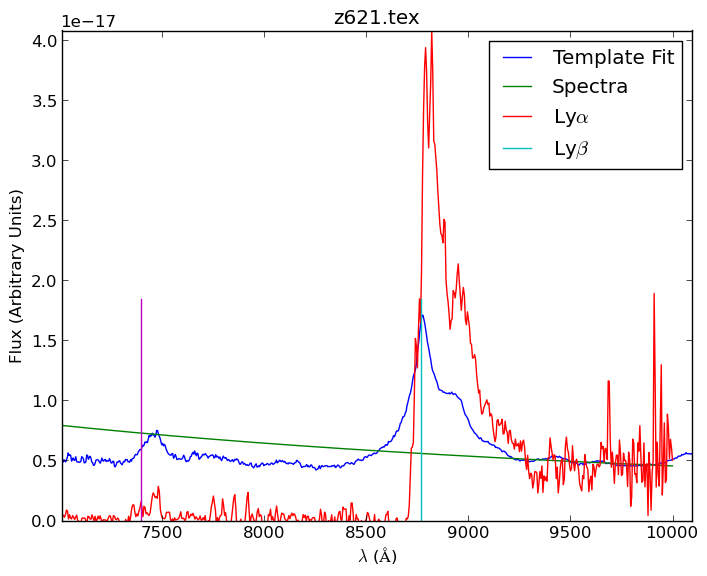
\includegraphics[width=8cm]{z621.png}
  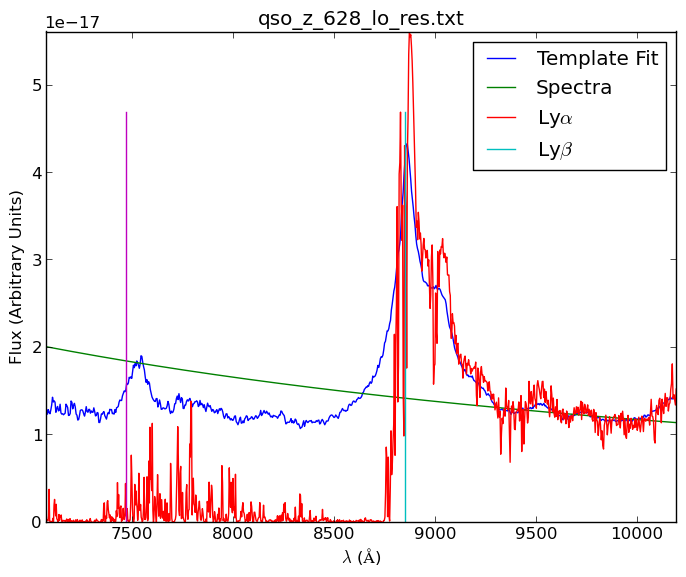
\includegraphics[width=8cm]{qso_z_628_lo_res.png}
  \caption{todo}
  \label{fig:todo}
\end{figure}

\begin{figure}[h]
  \centering
  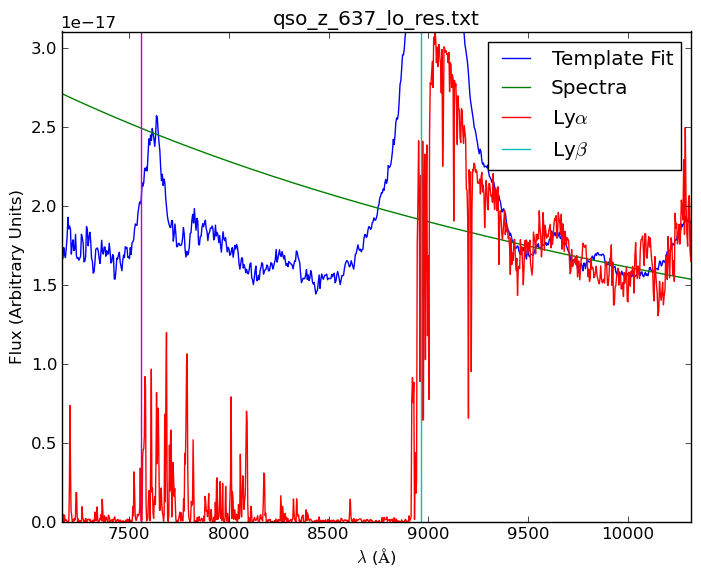
\includegraphics[width=8cm]{qso_z_637_lo_res.png}
  \caption{todo}
  \label{fig:todo}
\end{figure}


\end{document}